% Capítulo 3
\chapter{A matemática dos movimentos}
\label{ch:Math}

Para caminhar, Arash move suas juntas de uma forma sincronizada mantendo o equilíbrio. É um processo contínuo onde cada passo é planejado e possíveis perturbações são compensadas, o mais breve possível, afim de preservar a trajetória e evitar quedas.

O processo de caminhada é dividido em ciclos. Cada ciclo é dado pelo movimentos de passo da perna direita seguido pelo movimento da perna esquerda. O caminho percorrido pelos pés, suas posição e rotação, é predeterminado pelo \textit{walking gait} e é referido como trajetória.

A cada momento no tempo do ciclo -- levando em consideração também outras variáveis -- a trajetória fornece a posição e rotação de ambos os pés de Arash. A frequência de cada ciclo é definida por um relógio central definido no intervalo exibido na equação~\ref{eq:math:centraclock}, sendo $t$ o tempo do ciclo atual da caminhada.

\begin{equation}
	\label{eq:math:centraclock}
	0 \leq t < 2\pi
\end{equation}

No conceito de caminhada omnidirecional são utilizadas 3 velocidades afim de controlar a direção e velocidade do robô. $V_x$ é a velocidade em direção à frente, com valores positivos para a frente e negativos para caminhar de costas. $V_y$ é a velocidade lateral com onde passos para o lado são definidos com valores positivos implicando em movimentos laterais à direita. $V_\theta$ é a velocidade de rotação por passo com valores positivos indicando rotação também à direita.

Na figura~\ref{fig:math:velocities} é possível observar o diagrama com as posições dos pés e torso de Arash. Em azul estão ambos os pés e torso de Arash no início do ciclo de caminhada, quando $t$ é $0$. Em cinza, vê-se o pé direito e sua posição projetada quando $t$ vale $\pi$ (ou seja, metade do ciclo). Nota-se o deslocamento frontal em $V_x$, um deslocamento lateral em $V_y$ e um deslocamento angular em $V_\theta$ do torso, bem como do pé direito (afetado pela primeira metade do ciclo).

\begin{figure}[htb]
	\centering
	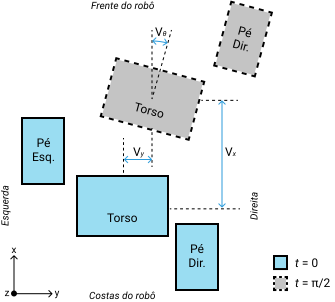
\includegraphics[scale=1]{imagens/svg/velocities-diagram}
	\caption{Diagrama da direção das velocidades da caminhada omnidirecional}
	\label{fig:math:velocities}
\end{figure}

Como mostra as equações~\ref{eq:math:velocities:intervals}, valores normalizados entre $-1.0$ e $1.0$ são utilizados para indicar as velocidades. Adotando-se $0.0$ como velocidade nula, ou sem movimento, $1.0$ como valor de velocidade máxima e $-1.0$ como valor de velocidade máxima no sentido oposto. Valores normalizados foram adotados para abstrair valores de velocidades absolutos já que futuras aplicações deste trabalho podem utilizar diferentes configurações de robôs. Desta forma, o controlador de comportamento pode abstrair a configuração do robô que está sendo controlado e enviando velocidades relativas. Adicionalmente, valores normalizados provém a integração perfeita entre as funções trigonométricas para a definição das trajetórias senoidais adotadas por \textit{Kamiri et al}.

\begin{equation}
\label{eq:math:velocities:intervals}
-1.0 \leq V_x \leq 1.0
\hspace{5mm},\hspace{5mm}
-1.0 \leq V_y \leq 1.0
\hspace{5mm},\hspace{5mm}
-1.0 \leq V_\theta \leq 1.0
\end{equation}

A cada iteração dois vetores $T$, de transferência, e $R$, de rotação, de cada pé são obtidos. Para o pé direito, utiliza-se o $t$ corrente no relógio central, já à perna esquerda um atraso de fase de $\pi/2$ é inserido.

A equação~\ref{eq:math:T_and_R:definition} mostra a definição de dos vetores $T$ e $R$. Cada um de seus elementos representam um eixo dentro deles e são gerados pelas trajetórias que são detalhadas na seção~\ref{sec:math:trajectories}.

\begin{equation}
\label{eq:math:T_and_R:definition}
T = [Foot_x,\hspace{3mm}Foot_y,\hspace{3mm}Foot_z],\hspace{5mm}R = [Foot_{roll},\hspace{3mm}Foot_{pitch},\hspace{3mm}Foot_{yaw}]
\end{equation}

Em poder desses vetores, utiliza-se os conceitos da cinemática inversa para gerar os ângulos de cada junta. Finalmente, os ângulos gerados são enviados aos motores -- como especificado na subseção~\ref{subsec:motors_abstraction} -- e, por fim, a iteração é finalizada.

\section{Orientação}
\label{sec:math:orientation}

Durante a implementação deste trabalho, nenhuma modificação foi realizada no componente de orientação originalmente desenvolvido por Kamiri \textit{et al}. Entretanto, para a implementação do cálculo da trajetórias é necessário algumas informações sobre a saída deste componente.

No final do processamento, obtém-se como saída um vetor com de aceleração linear nos eixos $x$ e $y$, como mostra a equação~\ref{eq:orientation:accel:definition}. Então, o vetor $Accel$ é utilizado para o cálculo da detecção de ``empurrões'', ou distúrbios, como visto nas equações \ref{eq:orientation:push:x} e \ref{eq:orientation:push:y}, que representação a variação na aceleração linear entre a iteração atual e a anterior.

\begin{align}
	Accel &= [Accel_x \hspace{5mm} Accel_y] \label{eq:orientation:accel:definition}
\end{align}

\begin{align}
	Push_x &= Accel[x]_t - Accel[x]_{t-1} 	 \label{eq:orientation:push:x}   \\
	Push_y &= Accel[y]_t - Accel[y]_{t-1}     \label{eq:orientation:push:y}
\end{align}

\section{Geração da trajetória}
\label{sec:math:trajectories}

Como afirmado anteriormente, a trajetória define a posição e rotação de ambos os pés de Arash durante cada momento do ciclo de caminhada, gerando como saída dois vetores $T$ e $R$, como definido na equação~\ref{eq:math:T_and_R:definition}. Kamiri \textit{et al} definem as funções que determinam cada eixo dos vetores, da equação \ref{eq:math:trajectories:foot:x} até \ref{eq:math:trajectories:foot:yaw}.

\begin{align}
      Foot_x &= \bigg(\dfrac{-cos(t) + 1}{2}\bigg) \times \bigg(\dfrac{tanh(V_x + Push_x) + H_{leg}}{\pi}\bigg)                    \label{eq:math:trajectories:foot:x}  \\
      Foot_y &= \big((-sin(t) \times B_{swing}) + (cos(t) + 1)\big) \times \bigg(\dfrac{tanh(V_y + Push_y) + H_{leg}}{2\pi}\bigg) \\
      Foot_z &= \bigg(\dfrac{sin(t)}{t + 1/2}\bigg) \times \bigg(\dfrac{tanh(V_x + V_y) \times H_{leg}}{\pi}\bigg) \\
 Foot_{roll} &= 0 \\
Foot_{pitch} &= 0 \\
  Foot_{yaw} &= \bigg(\dfrac{sin(V_\theta) + 1}{2}\bigg) \times \bigg(\dfrac{-cos(t) + 1}{2} \times V_\theta\bigg)     \label{eq:math:trajectories:foot:yaw}
\end{align}

Onde $t$ representa o tempo atual normalizado em cada ciclo; $B_{swing}$ representa a quantidade de compensação de balanço lateral que o corpo deve efetuar para compensar a dinâmica do movimento das pernas; $Push$ -- definido na seção~\ref{sec:math:orientation} -- é a quantidade de distúrbio causado por desvios na trajetória; por fim, $H_{leg}$ é o valor do tamanho da perna, extraído da estrutura do robô.

Nota-se que as funções $Foot_{roll}$ e $Foot_{pitch}$ são definidas como $0$ pois, em resultados experimentais, os efeitos durante a caminhada mostraram-se desprezíveis \cite{karimionline}.

\section{Cinemática Inversa}

Descobrir a posição de um parte do robô a partir dos ângulos de suas juntas, \textit{forward kinematics}, é uma tarefa fácil e pode ser realizada eficientemente. Porém, o oposto -- dado um ponto e calcular os ângulos das juntas que o alcancem; processo conhecido como \abrv[IK -- conhecido como \textit{Inverse Kinematics}, ou cinemática inversa]{IK (do inglês \textit{inverse kinematics} ou cinemática inversa)}-- não é uma tarefa tão simples.

Enquanto a problemas envolvendo a \textit{forward kinematics} possuem uma solução única, na \textit{IK} podem haver múltiplas soluções ou nenhuma \cite{spong2005robot}. Pode-se observar este fato ao tocar a ponta do próprio nariz, já que existem diversas combinações de posições do ombro, cotovelo, pulso e falanges que resolvem este problema; Entretando, usando as configurações de braço de um Tiranossauro o problema não teria solução, uma vez que o braço é demasiado curto para efetuar tal tarefa.

Aplicando a teoria da cinemática inversa ao problema proposto, Kamiri \textit{et al} apresenta uma solução direta aproveitando-se das limitações impostas pela configuração das juntas de Arash.

\begin{equation}
	\label{eq:math:ik:P:definition}
	P = [Hip_{yaw}, Hip_{roll}, Hip_{pitch}, Knee, Foot_{pitch}, Foot_{roll}] = iK(T, R)
\end{equation}

Na equação~\ref{eq:math:ik:P:definition}, vemos a definição do vetor P que mantém os valores dos ângulos de todas as juntas. Ele é a saída da função $iK$ que recebe como parâmetros os vetores $T$ e $R$ já definidos na equação~\ref{eq:math:T_and_R:definition}.

O processo de formulação das equações inicia-se a partir do nó principal do quadril descendo para o fim da cadeia, nos pés; onde encontra-se o fim da cadéia e o ponto de destino.

Na primeira etapa, a figura~\ref{fig:ik:upperview} mostra uma tomada de cima de Arash auxiliando na visualização da equação \ref{eq:ik:upper:hip:yaw}. Nota-se que, embora os pés de Arash não possuam rotação no eixo $yaw$ (figura~\ref{fig:architecture:arash:actuators_orientations}) a rotação $yaw$ aplicada no quadril, afeta toda a cadeia.

\begin{figure}[htb]
	\centering
	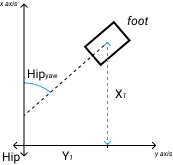
\includegraphics[scale=1.5]{imagens/svg/inverse-kinematics-upperview}
	\caption{Diagrama da visão superior da estrutura de Arash que representa da equação~\ref{eq:ik:upper:hip:yaw} até~\ref{eq:ik:upper:z:2}}
	\caption*{\cite{karimionline}}
	\label{fig:ik:upperview}
\end{figure}

\begin{align}
	P[Hip_{yaw}] &= R_{yaw}                             \label{eq:ik:upper:hip:yaw}  \\
	         X_2 &= T_x cos(R_{yaw}) + T_y sin(R_{yaw})  \label{eq:ik:upper:x:2}      \\
	         Y_2 &= -T_x sin(R_{yaw}) + T_ycos(R_{yaw})   \label{eq:ik:upper:y:2}      \\
	         Z_2 &= T_z                                    \label{eq:ik:upper:z:2}
\end{align}

Seguindo o processo de parametrização dos ângulos das juntas, observa-se na figura~\ref{fig:ik:frontalview} a visão frontal de Arash provendo uma visualização geométrica das equações~\ref{eq:ik:p:hip:roll} até \ref{eq:ik:z:3}. Nesta figura observa-se, também, o movimento no eixo $roll$ do quadril sendo compensado pelo movimento no sentido oposto (mas no mesmo eixo) do pé, afim de compensar o alinhamento do pé com o piso.

\begin{figure}[htb]
	\centering
	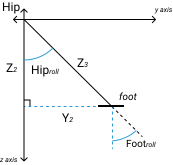
\includegraphics[scale=1.5]{imagens/svg/inverse-kinematics-frontalview}
	\caption{Diagrama da visão frontal de Arash que representa da equação~\ref{eq:ik:p:hip:roll} até~\ref{eq:ik:z:3}}
	\caption*{\cite{karimionline}}
	\label{fig:ik:frontalview}
\end{figure}

\begin{align}
	 P[Hip_{roll}] &= atan\bigg(\dfrac{Y_2}{Z_2}\bigg)                    \label{eq:ik:p:hip:roll}     \\
	P[Foot_{roll}] &= -P[Hip_{roll}] + R_{roll}                            \label{eq:ik:p:foot:roll}    \\
			   X_3 &= X_2                                                   \label{eq:ik:x:3}            \\
			   Y_3 &= Y_2                                                    \label{eq:ik:y:3}            \\
	           Z_3 &= \sqrt{Y_2^{\hspace{1mm}2} + {Z_2}^{\hspace{1mm}2}}      \label{eq:ik:z:3}
\end{align}

Na terceira etapa, a figura~\ref{fig:ik:frontalview} mostra a visão frontal de Arash, também, provendo uma visualização geométrica das equações~\ref{eq:ik:p:hip:roll} até \ref{eq:ik:z:3}.

\begin{figure}[htb]
	\centering
	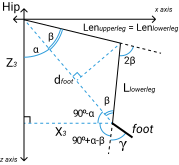
\includegraphics[scale=1.5]{imagens/svg/inverse-kinematics-sideview}
	\caption{Diagrama da visão lateral de Arash que representa da equação~\ref{eq:ik:p:hip:roll} até~\ref{eq:ik:z:3}}
	\caption*{\cite{karimionline}}
	\label{fig:ik:sideview}
\end{figure}

\begin{align}
	       d_{foot} &= \sqrt{Z_3^{\hspace{1mm}2} + X_3^{\hspace{1mm}2}}     \label{eq:ik:d:foot}        \\
	         \alpha &= atan\bigg(\dfrac{X_3}{Z_3}\bigg)                      \label{eq:ik:alpha}         \\
	          \beta &= acos\bigg(\dfrac{d_{foot}}{2 \times Leg_{len}}\bigg)   \label{eq:ik:beta}          \\
	 P[Hip_{pitch}] &= \alpha + \beta                                          \label{eq:ik:p:hip:pitch}   \\
	        P[Knee] &= -2 \beta                                                 \label{eq:ik:p:knee}        \\
	P[Foot_{pitch}] &= \gamma = -\alpha + \beta + R_{pitch}                      \label{eq:ik:p:foot:pitch}
\end{align}

Adicionalmente, a cada junta é somado um parâmetro de deslocamento -- não incluso nas equações de \textit{IK} --, também conhecido como \textit{offset}, para compensar possíveis erros provenientes de desalinhamentos no momento de montagem do robô, ou folgas nas engrenagens dos atuadores.

Finalmente, com as equações de \textit{IK} definidas, o \textit{walking gait}, com o auxílio dos componentes de orientação e \textit{proxy}, é apto a fazer os cálculos necessários para determinar os movimentos de caminhada.
